\documentclass[conference,a4paper]{IEEEtran}

\usepackage[T1]{fontenc}
\usepackage[utf8]{inputenc}
\usepackage{amsmath,amssymb}
\usepackage{balance}
\usepackage{booktabs}
\usepackage{cite}
\usepackage{graphicx}
\usepackage{tikz}
\usepackage{url}
\usetikzlibrary{arrows.meta,positioning}
\graphicspath{{paper/figures/}{paper/figures/generated/}}

\title{GeoZigzag Studio: A Reproducible Workflow for Agricultural Coverage and Semantic Georouting}

\author{
\IEEEauthorblockN{Luis Prieto-Lopez, Sergio Sanchez de La Fuente,
Miguel A. Gonzalez-Santamarta}
\IEEEauthorblockN{Angel Manuel Guerrero-Higueras, Lidia Sanchez-Gonzalez,
Francisco J. Rodriguez-Lera}
\IEEEauthorblockA{University of Leon, Leon, Spain\\
\texttt{luisprietolopez@protonmail.com}}
}

\begin{document}
\maketitle

\begin{abstract}
Agricultural mission preparation spans two different spatial tasks: dense
coverage of a field and sparse travel between geographically referenced
targets. Existing workflows commonly prepare these tasks in separate tools,
which complicates parameter tracking, route comparison, validation, and robot-
oriented export. This paper presents GeoZigzag Studio, a reproducible workflow
that combines boustrophedon coverage planning with semantic georouting in one
web interface and Python evaluation package. Semantic georouting is defined as
routing an ordered set of georeferenced targets while semantic land-cover
labels influence path cost or validity. The implementation formalizes local
projection, sweep-line coverage, direct interpolation, semantic-cost A$^\ast$,
forbidden-zone checks, optional OSRM routing, heading generation, and ROS-style
CSV/YAML export. A fixed-seed benchmark evaluates three fields and three
mission scenarios. The fields span 141--3289~m$^2$ and generate 224--710
waypoints. Across routing scenarios, direct paths intersect 4--7 forbidden-zone
segments; cost-aware paths reduce this count to zero with 4.6--7.3\% additional
distance. Cached OSRM routes expose maximum input-to-network snap distances of
35.2--90.8~m, demonstrating why network routes require explicit validation.
The repository provides offline tests, versioned scenarios, cached service
responses, generated figures and tables, and a single reproduction command.
\end{abstract}

\begin{IEEEkeywords}
agricultural robotics, coverage path planning, geospatial routing,
reproducibility, waypoint preparation, ROS~2
\end{IEEEkeywords}

\section{Introduction}
Agricultural mobile robots operate at more than one spatial scale. Within a
plot, sensing or treatment requires dense parallel passes. Between plots or
resources, the mission is instead a sparse sequence of targets such as water
points, crop areas, or access tracks. Coverage path planning (CPP) and
geographic routing address these needs, but their inputs, controls, and output
formats differ. Transferring a mission between tools can silently change
coordinate order, sampling density, target order, or assumptions about
traversability.

This separation also weakens experimental traceability. A screenshot alone
does not identify the algorithm, route parameters, map state, or external
service response that produced it. A research workflow should regenerate its
routes, metrics, tables, and figures from versioned inputs. It should also
distinguish a route that is geometrically valid from one that has been executed
successfully by a robot.

GeoZigzag Studio addresses this preparation layer. It combines interactive
field editing and mission ordering with a deterministic Python core. We use
\emph{semantic georouting} to mean: given an ordered sequence of sparse WGS84
targets and a spatial semantic model, compute a connecting route for which
labels such as track, shrub, or water modify traversal cost or admissibility.
This differs from CPP, whose objective is dense traversal of a bounded area,
and from local robot navigation, which closes the loop using localization and
perception.

The contributions are:
\begin{itemize}
  \item a unified, explicit workflow for dense field coverage and sparse
  semantic mission routing;
  \item formal algorithms for projection, coverage, cost-aware routing,
  forbidden-zone validation, and ROS-oriented orientation export;
  \item a multi-scenario benchmark comparing direct, semantic-cost, and cached
  OSRM routes using distance, waypoints, turns, time, intersections, snap
  distance, and success rate; and
  \item a reproducibility package with 20 offline tests, scenario files,
  service fixtures, generated artifacts, and \texttt{make reproduce}.
\end{itemize}

\section{Related Work and Research Gap}
CPP surveys describe decomposition and back-and-forth patterns for complete
area traversal~\cite{choset2001coverage,galceran2013survey}. Agricultural CPP
must additionally consider field shape, working width, headlands, and vehicle
turning constraints~\cite{oksanen2009coverage,hoffmann2024guidance}. The
Fields2Cover library provides reusable swath, route, and path components and a
benchmarking basis~\cite{mier2023fields2cover}. Nilsson and Zhou proposed 54
standard fields and agronomic measures for systematic comparison
~\cite{nilsson2020benchmark}. GeoZigzag does not replace these richer
vehicle-aware planners; it provides a lighter mission-preparation and
reproduction layer.

General GIS tools such as QGIS can construct saved chains of vector and raster
operations through the Processing Modeler~\cite{qgisModeler}. OSMnx automates
acquisition, projection, analysis, and routing over OpenStreetMap networks
~\cite{boeing2017osmnx}, while OSRM exposes network route and nearest services
and reports the distance from an input coordinate to its snapped network
location~\cite{osrmApi}. These tools are powerful, but they do not by
themselves provide the combined agricultural coverage, semantic mission, and
ROS-style export workflow considered here.

At execution time, Navigation2 provides ROS~2 planning and control and a
waypoint-follower action~\cite{macenski2020marathon2,macenski2022ros2}. It
expects a configured robot, frames, localization, costmaps, and controllers;
it is a downstream consumer rather than a geographic authoring environment.
Table~\ref{tab:comparison} locates the gap. ``P'' means possible through
configuration or plugins but not a first-class workflow; ``ROS'' denotes
waypoint export or consumption, not validated execution.

\begin{table}[t]
\caption{Workflow-level capability comparison.}
\label{tab:comparison}
\centering
\scriptsize
\begin{tabular}{lcccccc}
\toprule
Tool & CPP & Sem. & Web & Zones & ROS & Repro.\\
\midrule
Fields2Cover & Y & -- & -- & P & P & Y\\
QGIS & P & P & -- & Y & -- & Y\\
OSMnx/OSRM & -- & Y & P & P & -- & Y\\
Nav2 waypoint follower & -- & -- & -- & Y & Y & P\\
GeoZigzag Studio & Y & Y & Y & Y & Y & Y\\
\bottomrule
\end{tabular}
\end{table}

\section{System and Reproducible Workflow}
Figure~\ref{fig:architecture} shows the software boundary. Inputs are (i) a
WGS84 field polygon or labelled rectangle, (ii) row direction and start
corner, (iii) positive row and waypoint spacings, (iv) an ordered set of WGS84
targets with semantic labels, (v) optional forbidden polygons, and (vi) a
routing strategy. Outputs are the sampled route, yaw and planar quaternion at
each point, CSV/YAML/GeoJSON files, validation status, metrics, and provenance.

\begin{figure}[t]
\centering
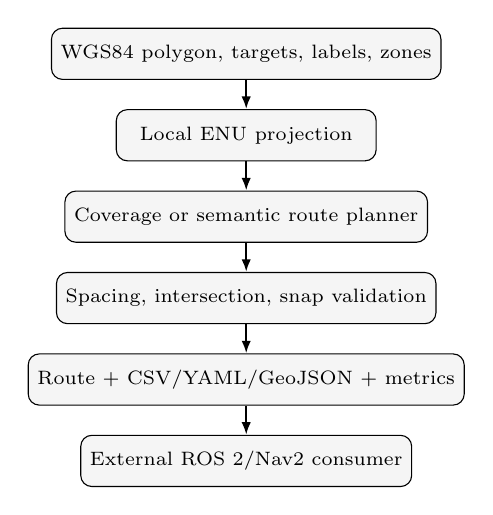
\begin{tikzpicture}[
  font=\scriptsize,
  node distance=3.7mm,
  box/.style={draw,rounded corners,align=center,fill=gray!8,minimum width=33mm,minimum height=6.5mm},
  arrow/.style={-{Latex[length=1.6mm]},thick}
]
\node[box] (input) {WGS84 polygon, targets, labels, zones};
\node[box,below=of input] (projection) {Local ENU projection};
\node[box,below=of projection] (planner) {Coverage or semantic route planner};
\node[box,below=of planner] (validation) {Spacing, intersection, snap validation};
\node[box,below=of validation] (export) {Route + CSV/YAML/GeoJSON + metrics};
\node[box,below=of export] (consumer) {External ROS~2/Nav2 consumer};
\draw[arrow] (input)--(projection);
\draw[arrow] (projection)--(planner);
\draw[arrow] (planner)--(validation);
\draw[arrow] (validation)--(export);
\draw[arrow] (export)--(consumer);
\end{tikzpicture}
\caption{GeoZigzag preparation pipeline. The external consumer is not part of
the route-generation evaluation.}
\label{fig:architecture}
\end{figure}

The Leaflet interface makes generation explicit. Editing a field, spacing,
target order, strategy, or forbidden zone marks the route \emph{pending},
disables stale downloads, and does not silently regenerate. Generation ends in
success, warning, or error state. OSRM warnings show the maximum snap distance;
intersection failures and fallback details remain visible to the operator.
Figure~\ref{fig:ui} shows both preparation modes.

\begin{figure*}[t]
\centering
\begin{minipage}[t]{0.485\textwidth}
\centering

\includegraphics[width=\linewidth]{coverage_ui.png}\\[-1mm]
\scriptsize (a) Coverage field, row controls, preview, and export.
\end{minipage}\hfill
\begin{minipage}[t]{0.485\textwidth}
\centering

\includegraphics[width=\linewidth]{mission_costmap_ui.png}\\[-1mm]
\scriptsize (b) Ordered targets, forbidden zone, status, and routing controls.
\end{minipage}
\caption{The two GeoZigzag Studio route-preparation modes. Both use explicit
generation, a shared route summary, visible validation state, and the same
waypoint export schema.}
\label{fig:ui}
\end{figure*}

\subsection{Operator Workflow}
In coverage mode, the operator draws or edits a rectangle or free polygon,
selects a start corner and row bearing, and sets row and waypoint spacing.
These two spacings remain independent: the former changes the agricultural
swaths, while the latter changes the sampling density of the exported route.
The field and previous route remain visible while parameters are edited, but
exports are marked stale until generation is requested again.

In mission mode, the operator creates an ordered sequence from GeoJSON targets
or custom map points and selects direct, semantic-cost, or OSRM routing. Manual
forbidden polygons encode areas that must be checked during preparation. An
OSRM result is accompanied by its snap-distance warning; a cost-aware failure
is reported rather than replaced silently by a direct segment.

After generation, the map provides the spatial sanity check, the summary shows
route-scale metrics, and the status block distinguishes success, warning, and
error. CSV is intended for inspection and analysis, YAML for ROS-oriented
consumers, and GeoJSON for independent GIS verification. The experiment runner
uses the same planners and schemas without the browser, binding every reported
result to a versioned scenario configuration.

\section{Methods}
\subsection{Projection, Heading, and Orientation}
For field-scale geometry, all input coordinates remain WGS84 while computation
uses a local equirectangular ENU approximation. For latitude--longitude
$(\phi,\lambda)$ and origin $(\phi_0,\lambda_0)$ in radians,
\begin{equation}
x=R\cos\phi_0(\lambda-\lambda_0),\quad y=R(\phi-\phi_0),
\end{equation}
with $R=6{,}378{,}137$~m, $x$ east, and $y$ north. The origin is the first
polygon point for coverage and the mean input coordinate for routing. This
approximation is used only for the sub-kilometre scenarios evaluated here.

For consecutive local points $p_i,p_{i+1}$, ROS ENU yaw is
$\psi_i=\operatorname{atan2}(\Delta y,\Delta x)$ normalized to
$[-\pi,\pi]$. The final point reuses the previous yaw. Exported planar
orientation is $(q_x,q_y,q_z,q_w)=(0,0,\sin(\psi/2),\cos(\psi/2))$.

\subsection{Coverage Planner}
The sweep direction is selected explicitly or inferred from the longest
polygon edge. Perpendicular sweep lines are separated by row spacing $s_r$.
Each line is intersected with every polygon edge; sorted intersections are
paired into valid in-field intervals. Samples along an interval are no farther
apart than waypoint spacing $s_w$. Traversal direction alternates by sweep.

\begin{figure}[t]
\footnotesize
\begin{minipage}{0.96\columnwidth}
\textbf{Algorithm 1: Polygon zigzag coverage}\\
1: validate polygon, $s_r>0$, and $s_w>0$\\
2: project vertices to local ENU and choose sweep axes\\
3: \textbf{for} $d=\min d_\perp$ to $\max d_\perp$ in steps $s_r$\\
4: \quad intersect line $d$ with all polygon edges\\
5: \quad sort intersections and pair inside intervals\\
6: \quad sample each interval at maximum spacing $s_w$\\
7: \quad append samples forward/reverse on alternating sweeps\\
8: attach yaw/quaternion; return route and coverage metrics
\end{minipage}
\end{figure}

The implementation reports polygon area, row count, mean clipped row length,
waypoint count, route distance, and discrete turns. A ``turn'' is a heading
change of at least $30^\circ$; it is a polyline metric, not a claim of
kinematic feasibility.

\subsection{Semantic and Network Routing}
Direct routing samples straight segments between ordered targets. Cost-aware
routing rasterizes all inputs on an 8-connected local grid. The evaluated
resolution is 4--5~m. A semantic point influences a radius of two cells (four
for water), using costs $1,1.5,10,30,80,1000$ for road, track, grass, shrub,
scrub, and water. Forbidden polygon cells receive infinite cost. For a path
$P=(v_0,\ldots,v_n)$, A$^\ast$ minimizes
\begin{equation}
J(P)=\sum_{k=1}^{n} c(v_k)\,\ell(v_{k-1},v_k),
\end{equation}
where $\ell$ is one or $\sqrt{2}$ grid steps. The admissible heuristic is
$c_{\min}$ times Euclidean cell distance. Failure to connect a target pair is
reported; there is no silent direct-route fallback.

For optional network routing, the OSRM route service returns a network
geometry and snapped waypoint records. GeoZigzag records
$d_{\mathrm{snap}}=\max_i d(g_i,\hat g_i)$ and rejects results above a
configured threshold. The offline benchmark uses a versioned response cache,
not a live service, so results do not change with network availability or OSM
updates.

\begin{figure}[t]
\footnotesize
\begin{minipage}{0.96\columnwidth}
\textbf{Algorithm 2: Semantic/cost-aware mission route}\\
1: validate ordered targets, resolution, labels, and zones\\
2: project inputs; build padded local cost grid\\
3: assign semantic costs; mark forbidden cells $\infty$\\
4: \textbf{for each} consecutive target pair $(g_i,g_{i+1})$\\
5: \quad run 8-connected A$^\ast$ using cost $J$\\
6: \quad \textbf{if} no path: return explicit failure\\
7: \quad restore exact target endpoints and concatenate\\
8: test every route segment against every zone edge\\
9: attach orientation; export route, validation, and metrics
\end{minipage}
\end{figure}

Forbidden-zone validation counts each route segment that lies inside, touches,
or crosses at least one polygon. It combines endpoint-in-polygon tests with
orientation-based segment intersection, including collinear contact. A route
is valid with respect to declared zones only when this count is zero.

\subsection{Validation State and Failure Semantics}
Let $H(P,\mathcal{Z})$ be the number of segments in route $P$ that intersect
any polygon in the declared zone set $\mathcal{Z}$, and let $S(P)$ be the
maximum OSRM snap distance when network routing is used. Given configured snap
limit $S_{\max}$, the route-level acceptance predicate is
\begin{equation}
\mathcal{V}(P)=\bigl[|P|\geq2\bigr]\land
\bigl[H(P,\mathcal{Z})=0\bigr]\land
\bigl[S(P)\leq S_{\max}\bigr].
\end{equation}
The snap term is omitted for local routes. This predicate describes only the
declared planning constraints; it is not a physical safety certificate.

The software distinguishes four states. \emph{Pending} means an input changed
after the last generation, so existing downloads are disabled. \emph{Success}
means the selected planner returned a route satisfying its configured checks.
\emph{Warning} preserves an inspectable result while exposing conditions such
as nonzero but permitted snap distance. \emph{Error} returns no current export
when spacing is invalid, geometry is degenerate, targets are missing, a route
is impossible, or a required service response is unavailable. The status and
detailed reason are stored separately so the main map remains readable without
hiding the failure cause.

Export occurs only from a non-pending generated state. CSV and YAML contain the
same WGS84, yaw, and quaternion values; GeoJSON adds a route line and indexed
point features. This one-to-one schema permits programmatic equality checks
across formats and prevents a browser preview from diverging silently from the
files used in evaluation.

\section{Experimental Evaluation}
\subsection{Research Questions}
The benchmark is organized around four questions. \emph{RQ1}: do row spacing
and waypoint spacing produce distinguishable and predictable effects on
coverage geometry and serialization density? \emph{RQ2}: what distance and
path-complexity penalty is paid when declared forbidden zones are enforced?
\emph{RQ3}: how different are network-routed missions from exact-target direct
routes, particularly in input-to-network snap distance? \emph{RQ4}: can every
reported route, metric, figure, and table be regenerated offline from versioned
inputs?

These questions evaluate workflow behavior rather than ranking GeoZigzag
against full vehicle-aware CPP or navigation systems. RQ1 is addressed by the
coverage scenarios and sensitivity sweep; RQ2 by paired direct and cost-aware
routes; RQ3 by cached OSRM responses; and RQ4 by repeated execution, artifact
generation, and automated tests.

\subsection{Protocol}
The evaluation configuration fixes seed 20260703 and executes each primary
planner five times. Timing is the median wall-clock duration on an Intel
Core~i7-13700KF with Python~3.10; it excludes file export and plotting. Three
coverage scenarios represent a compact rectangle, a medium quadrilateral, and
an irregular five-vertex field. Their areas are 141.2, 932.0, and
3288.9~m$^2$. Three semantic scenarios use different target orders and manual
forbidden-zone layouts. Every routing scenario is evaluated with direct,
semantic-cost A$^\ast$, and cached OSRM routing. The OSRM driving responses
were captured on 3 July 2026 and retain their reported snap distances.

Metrics are waypoint count, distance, coverage rows, heading-change turns,
median computation time, forbidden-zone intersections, maximum OSRM snap
distance, and success rate. Coverage sensitivity crosses four row spacings
$(0.5,0.75,1.0,1.5)$~m with three waypoint spacings $(0.5,1.0,2.0)$~m.

\begin{table}[t]
\caption{Semantic routing scenario configuration. Target initials denote
water (W), shrub (A), grass (P), and scrub (M).}
\label{tab:routing-scenarios}
\centering
\scriptsize
\begin{tabular}{lcccc}
\toprule
Scenario & Order & Grid (m) & Sample (m) & Zones\\
\midrule
north-loop & W--A--W & 5 & 10 & 1\\
west--east & P--M--P & 5 & 10 & 1\\
hazard-crossing & P--M--W & 4 & 8 & 1\\
\bottomrule
\end{tabular}
\end{table}

\subsection{Results}
All 60 primary executions (12 planner--scenario combinations, five repeats)
completed, for 100\% software-level generation success. Coverage produced
224, 347, and 710 waypoints over 16, 27, and 36 rows, with route distances of
205.8, 682.0, and 1753.7~m. Median coverage computation remained below 1~ms on
the test machine.

\begin{table}[t]
\caption{Coverage results generated from the configured fields.}
\label{tab:coverage-results}
\centering
\scriptsize
\begin{tabular}{lrrrr}
\hline
Scenario & Area (m$^2$) & Rows & Points & Dist. (m) \\
\hline
compact\_rectangle & 141.2 & 16 & 224 & 205.8 \\
medium\_rectangle & 932.0 & 27 & 347 & 682.0 \\
irregular\_field & 3288.9 & 36 & 710 & 1753.7 \\
\hline
\end{tabular}

\end{table}

\begin{table*}[t]
\caption{Routing results generated by \texttt{make reproduce}. ``Hits'' counts
route segments intersecting declared forbidden zones.}
\label{tab:results}
\centering
\small
\begin{tabular}{llrrrrr}
\hline
Scenario & Strategy & Points & Dist. (m) & Turns & Hits & Time (ms) \\
\hline
north\_loop & direct & 54 & 518.2 & 1 & 4 & 0.05 \\
north\_loop & cost\_aware & 83 & 542.7 & 18 & 0 & 58.67 \\
north\_loop & osrm\_cached & 34 & 1552.0 & 11 & 1 & 0.02 \\
west\_east & direct & 54 & 522.8 & 1 & 5 & 0.05 \\
west\_east & cost\_aware & 98 & 546.8 & 12 & 0 & 22.66 \\
west\_east & osrm\_cached & 30 & 1125.2 & 6 & 0 & 0.02 \\
hazard\_crossing & direct & 42 & 314.7 & 1 & 7 & 0.04 \\
hazard\_crossing & cost\_aware & 66 & 337.7 & 16 & 0 & 82.21 \\
hazard\_crossing & osrm\_cached & 11 & 293.6 & 4 & 3 & 0.01 \\
\hline
\end{tabular}

\end{table*}

Table~\ref{tab:results} shows the routing comparison. Direct routing is the
shortest exact-target baseline but intersects declared zones. Cost-aware
routing eliminates every intersection, increasing distance by 4.7\%, 4.6\%,
and 7.3\% for north-loop, west--east, and hazard-crossing missions. Its larger
turn count exposes grid discretization and shows why these routes still require
smoothing or a local planner before execution.

Cached OSRM follows the mapped driving network rather than the straight
mission geometry. It is substantially longer in two scenarios and still
intersects zones in two. More importantly, maximum snap distance is 87.7,
90.8, and 35.2~m. Thus a successful HTTP response is not sufficient evidence
that a network route reaches an agricultural target. Figure~\ref{fig:routes}
visualizes this difference.

\begin{figure}[t]
\centering

\includegraphics[width=\columnwidth]{comparison_north_loop.png}
\caption{Direct, forbidden-zone-aware semantic-cost, cached OSRM, and overlay
views for the north-loop mission.}
\label{fig:routes}
\end{figure}

Sensitivity results in Fig.~\ref{fig:sensitivity} separate geometric coverage
from sampling density. Increasing row spacing from 0.5 to 1.5~m reduces rows
from 23 to 9 and distance from 291.1 to 120.6~m. At fixed 0.75~m row spacing,
changing waypoint spacing from 0.5 to 2.0~m changes exported points from 430 to
128 while preserving route distance (205.8~m to numerical precision).

\begin{figure}[t]
\centering

\includegraphics[width=\columnwidth]{sensitivity.png}
\caption{Sensitivity to row and waypoint spacing on the compact field.}
\label{fig:sensitivity}
\end{figure}

\subsection{Robustness and Negative Cases}
Table~\ref{tab:negative-tests} summarizes failure-oriented checks. They execute
offline and assert observable behavior, not only that an exception occurred.
In particular, an impossible cost-grid mission is rejected rather than
silently converted into a direct route, and an OSRM transport failure is
reported through the external-routing error contract.

\begin{table}[t]
\caption{Offline robustness checks and required outcomes.}
\label{tab:negative-tests}
\centering
\scriptsize
\begin{tabular}{ll}
\toprule
Input or event & Required outcome\\
\midrule
$s_r\leq0$ or $s_w\leq0$ & Reject before planning\\
Degenerate polygon & No coverage export\\
Target enclosed by a zone & Explicit no-route error\\
OSRM timeout/failure & External-service error\\
Edit after generation & Pending state; exports disabled\\
Excessive OSRM snap & Reject above configured limit\\
\bottomrule
\end{tabular}
\end{table}

\section{Discussion}
The experiments expose three workflow-level trade-offs. First, row spacing and
waypoint spacing are not interchangeable controls. Row spacing changes the
physical sweep geometry, route length, and number of turns; waypoint spacing
primarily changes serialization density. Reporting only waypoint count would
therefore confound two different design decisions.

Second, a shorter geographic route is not necessarily an admissible route.
Direct interpolation provides a useful lower bound on distance but crosses the
declared zones in all three routing scenarios. The cost-aware planner removes
those intersections at a measured distance penalty, while its additional
corners reveal the need for curvature-aware post-processing. Validation and
path quality must consequently be reported together.

Third, network routing introduces a different uncertainty. The OSRM service
successfully returned all cached routes, yet two routes were much longer than
the direct alternatives and snap distances reached 90.8~m. Keeping exact input
targets, snapped geometry, service provenance, and validation results separate
prevents a visually plausible map route from being mistaken for an executable
robot path.

\section{Reproducibility and Software Validation}
The command \texttt{make reproduce} runs 20 offline tests, the configured
evaluation, figure/table generation, and LaTeX compilation. Each successful
route is exported as CSV, YAML, and GeoJSON. The summary records the random
seed, configuration SHA-256 digest, fixture version, per-run success, and all
reported metrics. Tests cover rectangle and polygon coverage, invalid spacing,
yaw/quaternion conversion, direct and cost-aware routing, impossible routes,
forbidden intersections, export schemas, mocked OSRM success/failure, generated
files, and web-state contracts. Online map tiles and live OSRM are optional and
excluded from offline tests.

The Python modules separate geometry, coverage, routing, metrics, export, and
evaluation. The previous public API remains as a compatibility facade. This
keeps the web/CLI workflow stable while allowing each scientific component to
be exercised independently.

\begin{table}[t]
\caption{Versioned inputs and generated reproducibility artifacts.}
\label{tab:artifacts}
\centering
\scriptsize
\begin{tabular}{ll}
\toprule
Artifact & Reproducibility role\\
\midrule
\texttt{evaluation.yaml} & Scenarios, parameters, seed, repeats\\
\texttt{osrm\_fixture.json} & Cached geometry, source, date, snaps\\
\texttt{waypoints.*} & CSV/YAML route and orientation schema\\
\texttt{route.geojson} & Independent GIS route inspection\\
\texttt{results.csv} & Per-scenario metrics and success rate\\
\texttt{summary.json} & Config hash, provenance, full results\\
\texttt{figures/*.png} & Code-generated paper comparisons\\
\bottomrule
\end{tabular}
\end{table}

Visual verification is part of the protocol but not substituted for numeric
validation. Each generated GeoJSON route can be overlaid with its targets,
field boundary, and forbidden zones. This catches coordinate-order or origin
errors that may still produce syntactically valid CSV/YAML files. Conversely,
the intersection and snap metrics prevent a visually plausible screenshot from
being treated as sufficient evidence.

\subsection{Downstream ROS 2 and Simulation Boundary}
The export is a preparation contract, not a complete launch interface. A Nav2
consumer must convert WGS84 coordinates into its configured \texttt{map}
frame, preserve the exported orientation convention, and validate localization
and costmap assumptions. Likewise, camera-based crop-row control consumes
images and publishes velocity commands rather than geographic waypoints.

Repository inspection identified a feasible staged validation: generate a
Gazebo world with the selected geographic origin, spawn the agricultural robot,
verify camera, odometry, command, and TF interfaces, then alternate global
row-entry goals with local crop-row control. This experiment requires explicit
command arbitration and row-end transitions; it is kept separate from the
software benchmark so that preparation metrics are not presented as navigation
performance.

\newpage
\balance
\section{Limitations and Threats to Validity}
The semantic cost layer is a controlled proxy built from labelled point
neighborhoods, not a calibrated traversability map. The grid paths contain
discrete corners and do not enforce turning radius, headland width, vehicle
footprint, soil response, or dynamics. Manual forbidden zones are only as
complete as operator input. The local projection is appropriate for the short
routes studied here, not regional missions.

Cached OSRM data improve repeatability but cannot establish current network
quality. Live results may change, fail, or snap differently as OSM and server
profiles evolve. Timing values are machine-dependent and the scenario set is
too small for claims of general superiority. The benchmark measures route
preparation, not localization, control, obstacle avoidance, simulated
completion, or field performance. ROS~2 waypoint execution and camera-based
crop-row following require separate frame, topic, controller, and safety
validation. Future work should compare against Fields2Cover on standard field
sets and measure executed cross-track error, missed area, interventions,
completion time, and target arrival error in simulation and on a robot.

\section{Conclusion}
GeoZigzag Studio turns two commonly separated planning tasks into a measurable
and reproducible agricultural mission-preparation workflow. Dense
boustrophedon coverage and sparse semantic georouting share projection,
validation, orientation, export, and provenance. The evaluation demonstrates
three concrete findings: row and waypoint spacing affect different properties;
declared forbidden zones can be avoided at a measurable distance and
complexity cost; and OSRM snap distance must be reported rather than hidden.
The resulting artifact generates its routes, metrics, figures, and manuscript
tables from versioned inputs while keeping robot execution claims outside the
evidence provided.

\bibliographystyle{IEEEtran}
\bibliography{paper/references}

\end{document}
